\documentclass[onecolumn,conference]{IEEEtran}

\usepackage[letterpaper,margin=0.72in]{geometry}
\usepackage{graphicx}
\usepackage{amsmath}
\usepackage{booktabs}
\usepackage{cite}
\usepackage{url}
\usepackage{microtype}
\usepackage{caption}

\graphicspath{{figures/}}
\setlength{\parskip}{0.15em}
\setlength{\textfloatsep}{0.55em}
\setlength{\floatsep}{0.45em}
\setlength{\intextsep}{0.45em}

\title{A Fixed-Point FPGA Correlation Accelerator for Orthogonal Matching Pursuit}

\author{
    \IEEEauthorblockN{ENGS 109 Final Project}
    \IEEEauthorblockA{Dartmouth College\\
    \texttt{engs109-omp-fpga}}
}

\begin{document}
\maketitle

\begin{abstract}
Orthogonal Matching Pursuit (OMP) is a sparse recovery algorithm whose repeated dictionary-correlation step is a natural target for FPGA acceleration. This project implements and evaluates a fixed-point OMP correlation engine for a Zynq-7020-class FPGA system. The accelerator computes the inner product between a residual vector and all dictionary atoms, returns the atom index with maximum absolute correlation, and leaves the least-squares solve and residual update in software. A Python bit-accurate reference, golden vectors, a Cortex-A9 software baseline, and Vivado synthesis sweeps were used to verify correctness and study precision/resource tradeoffs. The final design target uses Q1.15 external data, a 128-sample measurement vector, 256 dictionary atoms, and up to 32 OMP iterations. Synthesis results show that the BRAM-backed fixed-point correlation engine can meet a 100 MHz target while using 16 BRAM tiles; MAC widths of 11 bits and above infer DSPs and reduce LUT count compared with LUT-only lower precision designs.
\end{abstract}

\section{Introduction}
Compressed sensing reconstructs sparse or compressible signals from fewer measurements than conventional sampling would require. OMP is a common greedy reconstruction method: at each iteration it chooses the dictionary atom most correlated with the current residual, solves a least-squares problem over the selected support, and updates the residual~\cite{mallat,tropp}. For an $M \times N$ dictionary, the correlation pass requires $N$ length-$M$ inner products every iteration, making it the most regular and parallel part of the algorithm.

The goal of this project was to build a hardware/software OMP system where the FPGA fabric accelerates the correlation pass and the processor handles control-heavy work. The selected system dimensions are $M=128$, $N=256$, window length 256, and maximum support size 32. The implementation uses Q1.15 fixed-point values at the hardware boundary and sweeps the internal multiply-accumulate input width, denoted \texttt{MAC\_BITS}, to explore the accuracy and resource cost of truncation.

\section{Background}
Given a measurement vector $y \in \mathbb{R}^{M}$ and dictionary $D \in \mathbb{R}^{M \times N}$, OMP approximates $y$ using a small set of atoms. At iteration $t$, the correlation step computes
\begin{equation}
    \lambda_t = \arg\max_j \left|D_j^T r_t\right|,
\end{equation}
where $D_j$ is the $j$th atom and $r_t$ is the current residual. The selected index is appended to the support set. Software then solves
\begin{equation}
    \hat{x}_{S_t} = \arg\min_z \left\|y - D_{S_t}z\right\|_2
\end{equation}
and updates $r_{t+1}=y-D_{S_t}\hat{x}_{S_t}$.

The correlation pass is well matched to hardware because it is dominated by repeated multiply-accumulate operations and a reduction tree. The least-squares solve is less attractive for a small course project accelerator because it has more data-dependent control, numerical corner cases, and lower arithmetic regularity at the chosen problem size. Splitting OMP this way keeps the FPGA block stateless with respect to the full support set while still accelerating the repeated kernel.

\section{System Design}
Fig.~\ref{fig:arch} shows the project architecture. The software side owns the OMP loop, quantization, least-squares solve, residual update, and reconstruction quality measurements. The FPGA block owns one operation: compute all atom correlations for the current residual and return the winning atom index and signed accumulator value. The hardware-visible parameters are fixed across the project: $M=128$, $N=256$, Q1.15 inputs, a 100 MHz clock, and up to 32 software-controlled OMP iterations on a Zynq-7000 target~\cite{xilinx}.

\begin{figure}[t]
    \centering
    \small
    \setlength{\fboxsep}{5pt}
    \begin{tabular}{c c c}
    \fbox{\parbox{0.25\linewidth}{\centering Offline Python\\ECG windows, db4 basis\\golden vectors}}
    & $\longrightarrow$ &
    \fbox{\parbox{0.25\linewidth}{\centering Zynq PS\\OMP loop, least squares\\residual update}} \\
    && $\downarrow$ \\
    \fbox{\parbox{0.25\linewidth}{\centering C baseline\\timed correlation pass\\PRD measurement}}
    & $\longleftarrow$ &
    \fbox{\parbox{0.25\linewidth}{\centering Programmable logic\\Q1.15 correlation engine\\argmax result}} \\
    \end{tabular}
    \caption{Hardware/software partition. The programmable logic accelerates the dictionary-residual correlation pass; the processor executes support management, least squares, residual updates, and final reconstruction.}
    \label{fig:arch}
\end{figure}

The fixed-point datapath stores dictionary and residual samples as signed Q1.15 values. For each atom, the engine computes
\begin{equation}
    a_j = \sum_{i=0}^{127} D_{i,j} r_i
\end{equation}
using integer arithmetic. The selected result is $\arg\max_j |a_j|$. The full-precision product of two Q1.15 values is Q2.30; summing 128 terms requires additional accumulator headroom, so the software model uses 64-bit integer arithmetic while the hardware reports a signed accumulator value sized for the design. Tie behavior is defined as lowest index wins, matching \texttt{numpy.argmax} and the C baseline's strict comparison.

\section{Methodology}
The project used a layered verification flow. First, a floating-point OMP implementation established an accuracy ceiling. Second, a bit-accurate fixed-point Python model implemented the exact hardware correlation operation, including optional arithmetic right shifts for \texttt{MAC\_BITS} truncation. Third, five golden-vector cases tested easy margins, tight margins, winners near index 0, winners near index $N-1$, and an engineered tie. These vectors are stored as \texttt{.npz} and \texttt{.mem} files for Python and HDL-side reuse.

The software baseline is a C implementation of OMP for the Cortex-A9 path. Only the correlation pass is timed because that is the kernel replaced by hardware. The baseline still runs the full OMP scaffold so that each recovered window produces a support set and percent root-mean-square difference (PRD),
\begin{equation}
    \mathrm{PRD}=100\frac{\left\|x-\hat{x}\right\|_2}{\left\|x\right\|_2}.
\end{equation}
The checked-in baseline results cover 120 windows with 32 selected atoms per window.

Finally, Vivado 2021.2 synthesis sweeps measured resource usage and timing for several \texttt{MAC\_BITS} values on an \texttt{xc7z020clg400-1} target. The sweep records slice LUTs, DSPs, BRAM tiles, worst negative slack, and estimated maximum frequency.

\section{Results}
The Cortex-A9 software reconstruction baseline produced a mean PRD of 20.13\%, median PRD of 16.51\%, minimum PRD of 9.01\%, and maximum PRD of 80.88\% across 120 windows. The high-PRD outliers indicate that reconstruction quality depends strongly on the selected window and dictionary coherence, so the hardware precision study should be interpreted as a tradeoff against an already imperfect sparse model rather than against exact reconstruction.

\begin{table}[t]
\centering
\caption{Vivado synthesis sweep for the correlation engine.}
\label{tab:sweep}
\begin{tabular}{rrrrrr}
\toprule
\texttt{MAC\_BITS} & LUT & DSP & BRAM & WNS (ns) & Fmax (MHz) \\
\midrule
3  & 867  & 0  & 16 & 2.780 & 138.5 \\
4  & 1473 & 0  & 16 & 2.780 & 138.5 \\
5  & 1760 & 0  & 16 & 2.780 & 138.5 \\
6  & 2078 & 0  & 16 & 2.780 & 138.5 \\
8  & 3034 & 0  & 16 & 2.780 & 138.5 \\
10 & 4503 & 0  & 16 & 1.162 & 113.1 \\
11 & 610  & 47 & 16 & 2.780 & 138.5 \\
12 & 610  & 47 & 16 & 2.780 & 138.5 \\
16 & 610  & 47 & 16 & 2.780 & 138.5 \\
\bottomrule
\end{tabular}
\end{table}

Table~\ref{tab:sweep} shows a clear implementation regime change. At 10 bits and below, the multipliers remain in LUT fabric and LUT count grows with precision. At 11 bits and above, Vivado infers 47 DSP blocks and the LUT count drops to 610. BRAM usage is constant at 16 tiles because it is dominated by dictionary/residual storage rather than arithmetic precision. All sweep points meet the 100 MHz target, but the 10-bit LUT-only point has the smallest timing margin. This makes the 11-bit DSP-backed design an attractive operating point: it preserves timing margin and reduces LUT pressure while avoiding full 16-bit multiplier cost in the datapath.

\begin{figure}[t]
    \centering
    
\includegraphics[width=0.82\linewidth]{resource_crossover.png}
    \caption{Resource crossover in the \texttt{MAC\_BITS} sweep. Lower widths use LUT arithmetic; 11 bits and above map to DSP resources and reduce LUT pressure.}
    \label{fig:crossover}
\end{figure}

Fig.~\ref{fig:pareto} summarizes the broader precision/resource tradeoff. Very low \texttt{MAC\_BITS} settings reduce arithmetic precision enough to damage atom selection. Once the width is high enough to preserve the dominant correlation ordering for typical residuals, additional precision gives diminishing reconstruction benefit while continuing to consume resources or DSP blocks. The project therefore emphasizes choosing the narrowest width that maintains acceptable support selection behavior.

\begin{figure}[t]
    \centering
    
\includegraphics[width=0.82\linewidth]{pareto_combined_betterExp.png}
    \caption{Combined Pareto view of reconstruction quality and hardware cost across precision settings.}
    \label{fig:pareto}
\end{figure}

The beat reconstruction example in Fig.~\ref{fig:recon} illustrates the end-to-end signal-level effect of the sparse recovery flow. The reconstructed waveform captures the dominant morphology but not every high-frequency detail, which is consistent with the finite support size and compressed measurement dimension.

\begin{figure}[t]
    \centering
    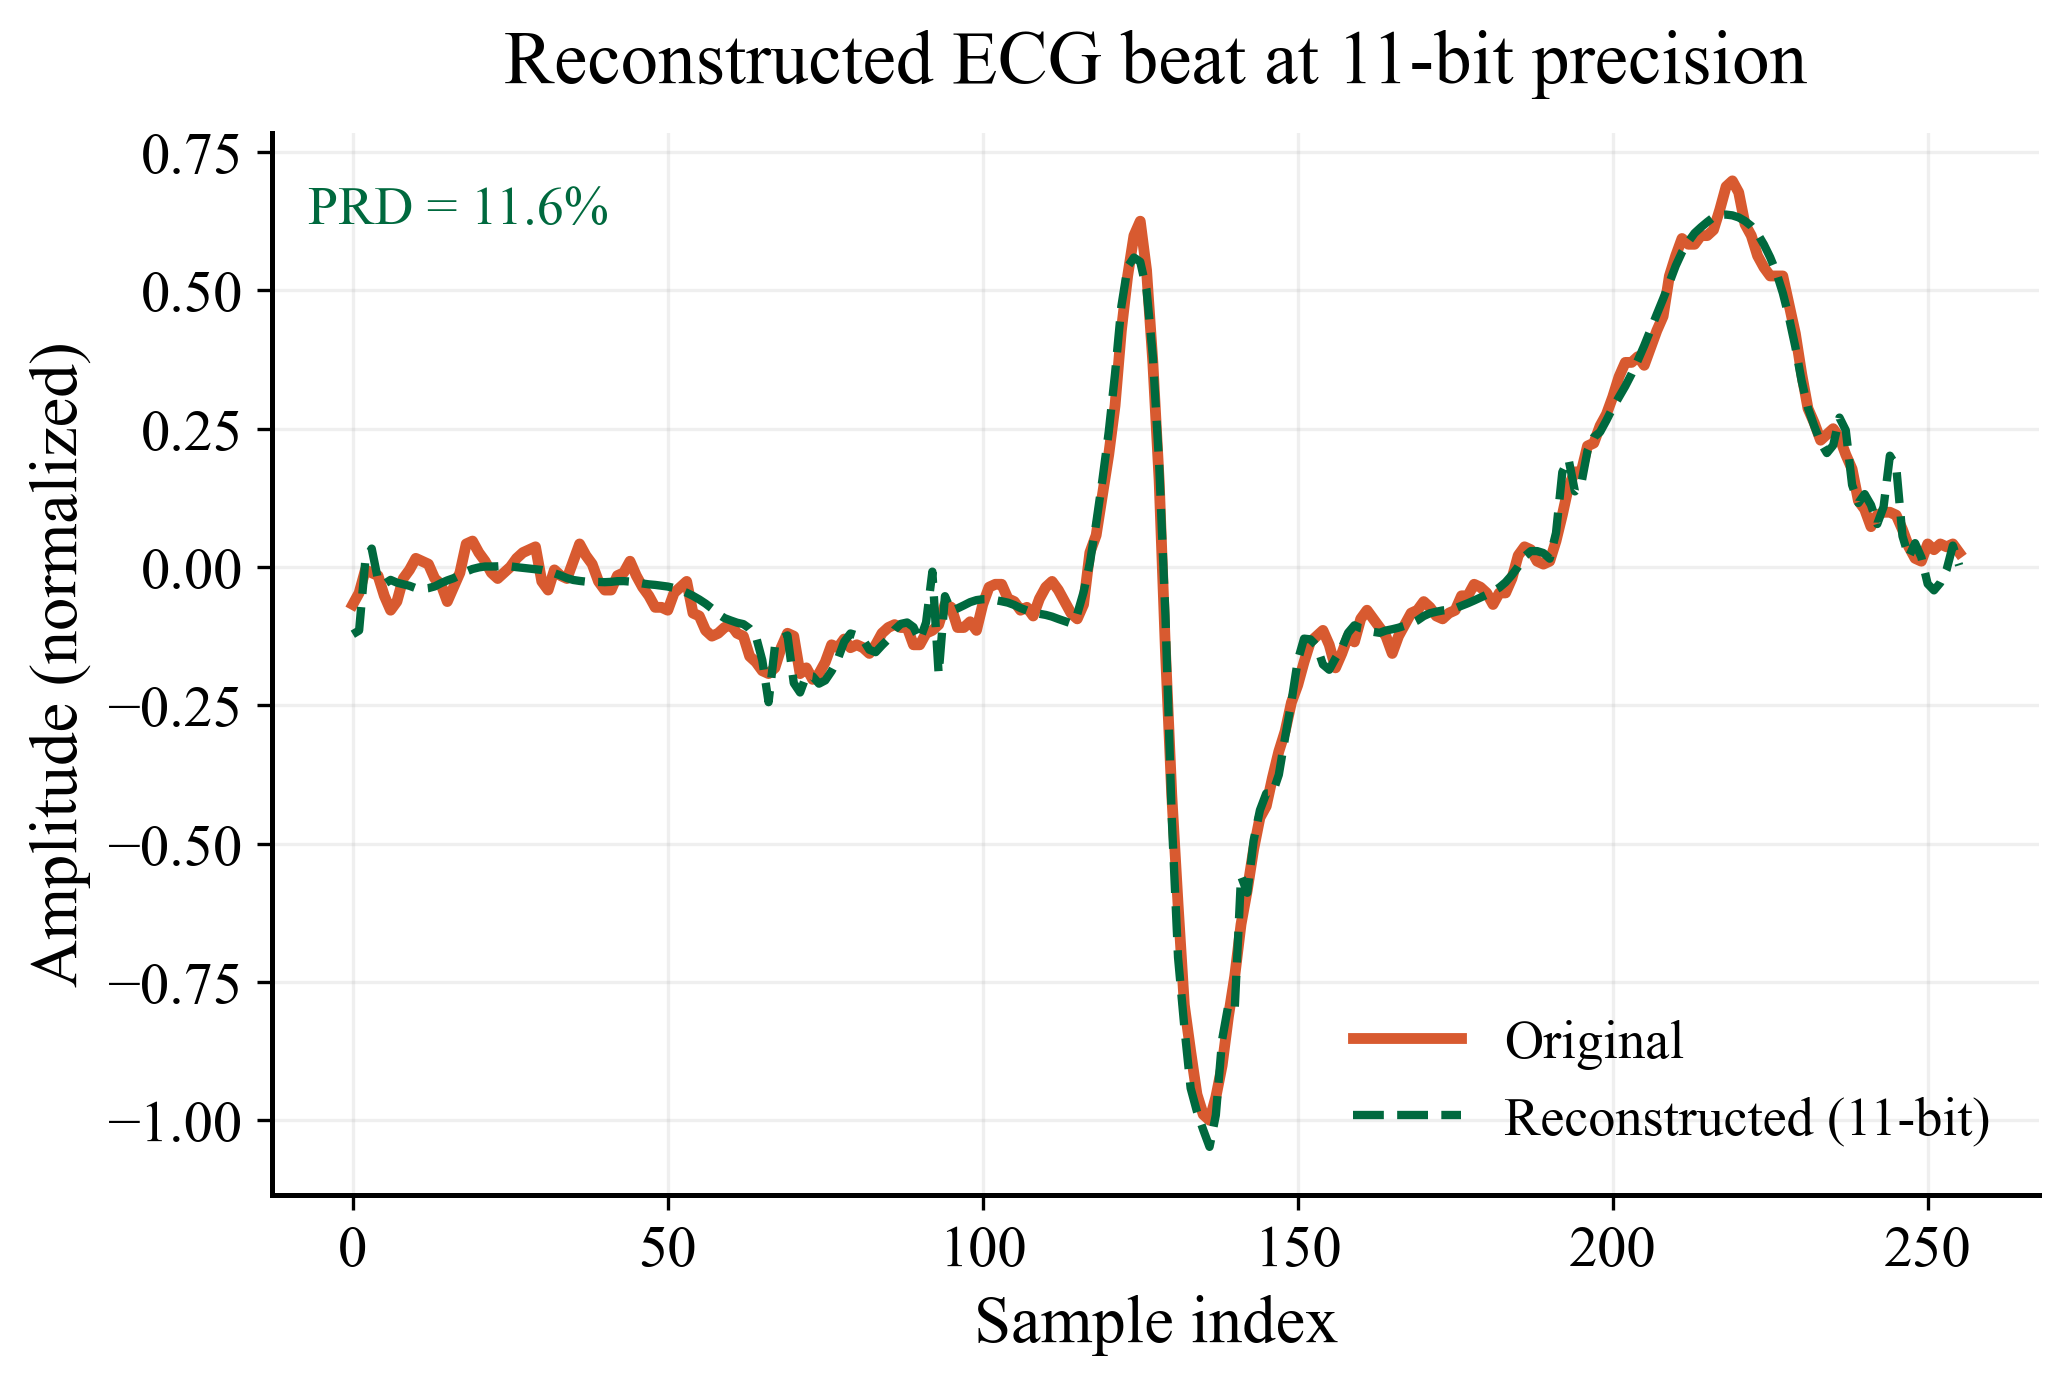
\includegraphics[width=0.86\linewidth]{recon_beat_11bit.png}
    \caption{Example reconstructed beat using the fixed-point OMP flow.}
    \label{fig:recon}
\end{figure}

\section{Discussion}
The main design decision was to accelerate only the correlation pass. This kept the hardware interface simple and allowed correctness to be tested independently with deterministic golden vectors. It also avoided moving the least-squares solve into fabric before the fixed-point correlation behavior was fully characterized. The tradeoff is that end-to-end acceleration is limited by processor-side residual updates and solves; future work would need board-level timing of the accelerator call overhead and possibly batching or DMA support to reduce communication cost.

The synthesis results also show that lower bit width does not automatically mean lower total cost. For this device and design, 11-bit arithmetic is cheaper in LUTs than 10-bit arithmetic because the synthesis tool changes multiplier mapping. This reinforces the need for empirical FPGA sweeps rather than relying only on bit-width intuition.

\section{Conclusion}
This project produced a verified fixed-point correlation accelerator path for OMP sparse recovery. The software reference, golden vectors, C baseline, and Vivado synthesis sweep together establish a reproducible methodology for evaluating correctness, reconstruction quality, and hardware cost. The most useful result is the precision/resource crossover: an 11-bit internal MAC setting meets timing at 100 MHz, uses 16 BRAM tiles and 47 DSPs, and reduces LUT usage to 610, making it a strong candidate for the final FPGA implementation. Future improvements should focus on hardware-in-the-loop timing, AXI transfer optimization, and extending acceleration beyond the correlation pass once the communication overhead is quantified.

\begin{thebibliography}{1}
\bibitem{mallat}
S. G. Mallat and Z. Zhang, ``Matching pursuits with time-frequency dictionaries,'' \emph{IEEE Transactions on Signal Processing}, vol. 41, no. 12, pp. 3397--3415, 1993.

\bibitem{tropp}
J. A. Tropp and A. C. Gilbert, ``Signal recovery from random measurements via orthogonal matching pursuit,'' \emph{IEEE Transactions on Information Theory}, vol. 53, no. 12, pp. 4655--4666, 2007.

\bibitem{xilinx}
AMD Xilinx, \emph{Zynq-7000 SoC Data Sheet: Overview}, DS190.
\end{thebibliography}

\end{document}
